% ============================================================
%  Project Documentation — Skin Lesion CAD System
%  Group 5 | Deep Learning Course
%  Baraa Lazkani & Humam Yehia
% ============================================================
\documentclass[12pt,a4paper]{report}

% --- Encoding & fonts ---
\usepackage[utf8]{inputenc}
\usepackage[T1]{fontenc}
\usepackage{lmodern}

% --- Layout ---
\usepackage[top=2.5cm,bottom=2.5cm,left=2.8cm,right=2.8cm]{geometry}
\setlength{\headheight}{15pt}
\usepackage{parskip}
\usepackage{setspace}
\onehalfspacing

% --- Graphics ---
\usepackage{graphicx}
\graphicspath{{./Analysis/outputs/}}

% --- Colour & hyperlinks ---
\usepackage{xcolor}
\definecolor{mainblue}{RGB}{30,90,160}
\definecolor{lightblue}{RGB}{220,235,250}
\definecolor{codered}{RGB}{180,30,30}
\definecolor{codebg}{RGB}{248,248,252}
\definecolor{codegreen}{RGB}{0,120,0}
\definecolor{codegray}{RGB}{120,120,120}
\definecolor{codepurple}{RGB}{140,0,200}

\usepackage[hidelinks,
            colorlinks=true,
            linkcolor=mainblue,
            urlcolor=mainblue,
            citecolor=mainblue]{hyperref}

% --- Tables ---
\usepackage{booktabs}
\usepackage{array}
\usepackage{longtable}
\usepackage{multirow}
\usepackage{tabularx}

% --- Code listings ---
\usepackage{listings}
\lstdefinestyle{pystyle}{
  backgroundcolor=\color{codebg},
  commentstyle=\color{codegreen}\itshape,
  keywordstyle=\color{mainblue}\bfseries,
  numberstyle=\tiny\color{codegray},
  stringstyle=\color{codepurple},
  basicstyle=\ttfamily\footnotesize,
  breakatwhitespace=false,
  breaklines=true,
  captionpos=b,
  keepspaces=true,
  numbers=left,
  numbersep=6pt,
  showspaces=false,
  showstringspaces=false,
  tabsize=4,
  language=Python,
  frame=single,
  framesep=4pt,
  rulecolor=\color{mainblue!40},
}
\lstset{style=pystyle}

% --- TikZ ---
\usepackage{tikz}
\usetikzlibrary{shapes.geometric,arrows.meta,positioning,fit,calc,backgrounds,decorations.pathreplacing}

% --- Misc ---
\usepackage{amsmath,amssymb}
\usepackage{caption}
\usepackage{subcaption}
\usepackage{enumitem}
\usepackage{fancyhdr}
\usepackage{titlesec}
\usepackage{tcolorbox}
\tcbuselibrary{skins,breakable}

% --- Chapter / section style ---
\titleformat{\chapter}[display]
  {\normalfont\huge\bfseries\color{mainblue}}
  {\chaptertitlename\ \thechapter}{14pt}{\Huge}
\titlespacing{\chapter}{0pt}{-10pt}{30pt}

\titleformat{\section}
  {\normalfont\Large\bfseries\color{mainblue!80!black}}
  {\thesection}{1em}{}
\titleformat{\subsection}
  {\normalfont\large\bfseries\color{mainblue!60!black}}
  {\thesubsection}{1em}{}

% --- Page style ---
\pagestyle{fancy}
\fancyhf{}
\lhead{\small\textit{Skin Lesion CAD System -- Documentation}}
\rhead{\small\textit{Group 5 | Deep Learning Course}}
\cfoot{\thepage}
\renewcommand{\headrulewidth}{0.4pt}

% --- Highlight box ---
\newtcolorbox{notebox}[1][]{
  enhanced,
  colback=lightblue,
  colframe=mainblue,
  fonttitle=\bfseries,
  title=#1,
  breakable,
  left=6pt, right=6pt, top=4pt, bottom=4pt,
}

% ============================================================
\begin{document}

% ==========================================================
%  TITLE PAGE
% ==========================================================
\begin{titlepage}
  \pagecolor{mainblue!10}
  \centering
  \vspace*{1.5cm}

  % Decorative top rule
  {\color{mainblue}\rule{\linewidth}{2pt}}\\[1em]

  {\fontsize{28}{36}\selectfont\bfseries\color{mainblue}
    A Cutting-Edge End-to-End System\\[6pt]
    for Skin Lesion Segmentation\\[6pt]
    and Classification\par}

  \vspace{0.6cm}
  {\color{mainblue}\rule{\linewidth}{2pt}}\\[2em]

  % Mini pipeline diagram
  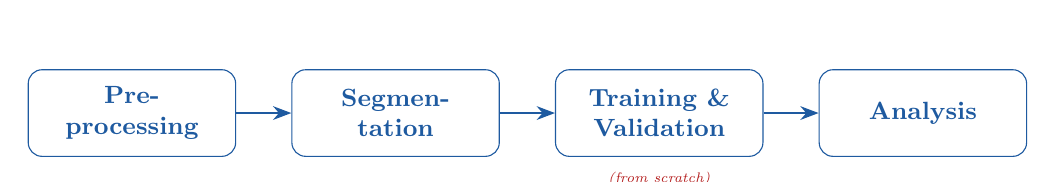
\begin{tikzpicture}[
    tbox/.style={rectangle, rounded corners=5pt,
                 draw=mainblue, fill=white,
                 minimum width=2.6cm, minimum height=1.1cm,
                 align=center, font=\small\bfseries\color{mainblue},
                 text width=2.4cm},
    arr/.style={-Stealth, thick, mainblue}
  ]
    \node[tbox] (p1) {Pre-\\processing};
    \node[tbox, right=0.7cm of p1] (p2) {Segmen-\\tation};
    \node[tbox, right=0.7cm of p2] (p3) {Training \&\\Validation};
    \node[tbox, right=0.7cm of p3] (p4) {Analysis};
    \draw[arr] (p1)--(p2);
    \draw[arr] (p2)--(p3);
    \draw[arr] (p3)--(p4);
    \node[font=\tiny\itshape, below=2pt of p3, text=codered] {(from scratch)};
  \end{tikzpicture}

  \vspace{2.5cm}

  {\LARGE\bfseries\color{mainblue} Group 5}\par
  \vspace{0.3cm}
  {\large Deep Learning Course}\par

  \vspace{1.5cm}

  \begin{tabular}{@{}ll@{}}
    {\bfseries Authors:}  & Baraa Lazkani \\
                          & Humam Yehia   \\[6pt]
    {\bfseries Dataset:}  & ISIC 2018 Task 3 \\
    {\bfseries Model:}    & DenseNet-121 (pure NumPy, from scratch) \\
    {\bfseries Date:}     & May 2026 \\
  \end{tabular}

  \vfill
  {\color{mainblue}\rule{\linewidth}{2pt}}
  \nopagecolor
\end{titlepage}

\nopagecolor

% ==========================================================
%  FRONT MATTER
% ==========================================================
\tableofcontents
\clearpage
\listoffigures
\listoftables
\clearpage

% ==========================================================
\chapter{Introduction and Project Overview}
% ==========================================================

\section{Motivation}

Skin cancer is among the most common cancers worldwide, and dermoscopy — the imaging of skin lesions through a dermatoscope — provides a non-invasive window into their structure. Accurate classification of dermoscopy images remains challenging even for trained dermatologists due to the subtle visual differences between benign and malignant lesions.

Computer-Aided Diagnosis (CAD) systems driven by deep learning have demonstrated remarkable potential in this domain. This project presents a complete end-to-end CAD pipeline for the \textbf{ISIC 2018 Task 3} benchmark, covering image enhancement, lesion segmentation, and multi-class classification.

\section{Original Contribution}

\begin{notebox}[Scope of Original Work]
The \textbf{Preprocessing \& Segmentation} phase (Phase 1) was provided as part of the project framework. The \textbf{Training \& Validation} phase (Phase 2) was designed and implemented \textbf{entirely from scratch} by the authors using pure \textbf{NumPy only} — no deep learning framework (PyTorch, TensorFlow, Keras, JAX, etc.) was used for the model, optimizer, loss, or data pipeline. This includes:
\begin{itemize}[nosep]
  \item A full DenseNet-121 forward and backward pass
  \item Custom convolution via \texttt{im2col}/\texttt{col2im}
  \item Batch Normalization, Dropout, Pooling layers
  \item Adam optimizer with bias correction
  \item Focal Loss with analytic gradient
  \item Cosine annealing and early stopping
  \item Weighted random sampling for class imbalance
\end{itemize}
The \textbf{Analysis} phase (Phase 3) post-processes the saved training logs and produces evaluation plots.
\end{notebox}

\section{Dataset: ISIC 2018 Task 3}

The International Skin Imaging Collaboration (ISIC) 2018 Task 3 provides labelled dermoscopy images across seven diagnostic categories. Table~\ref{tab:classes} shows the class distribution.

\begin{table}[ht]
  \centering
  \caption{ISIC 2018 Task 3 class distribution (training split)}
  \label{tab:classes}
  \begin{tabular}{llrp{6cm}}
    \toprule
    \textbf{Code} & \textbf{Full Name} & \textbf{Count} & \textbf{Description} \\
    \midrule
    MEL   & Melanoma                              & 1{,}113 & Malignant melanocytic tumour \\
    NV    & Melanocytic Nevi                      & 6{,}705 & Common benign mole \\
    BCC   & Basal Cell Carcinoma                  &   514   & Most common skin cancer \\
    AKIEC & Actinic Keratosis / Bowen's Disease   &   327   & Pre-malignant sun-damage lesion \\
    BKL   & Benign Keratosis-like Lesion          & 1{,}099 & Seborrheic keratosis \\
    DF    & Dermatofibroma                        &   115   & Benign fibrous skin nodule \\
    VASC  & Vascular Lesions                      &   142   & Angioma, angiokeratoma, etc. \\
    \midrule
    \multicolumn{2}{l}{\textbf{Total (usable)}} & \textbf{9{,}835} & \\
    \bottomrule
  \end{tabular}
\end{table}

The dataset is heavily imbalanced: NV alone accounts for $\approx$68\% of samples, while DF and VASC together represent fewer than 3\%. Addressing this imbalance is a key design concern in the training phase.

\section{Overall System Architecture}

Figure~\ref{fig:pipeline} shows the complete data and computation flow from a raw dermoscopy image to a classification decision.

\begin{figure}[ht]
  \centering
  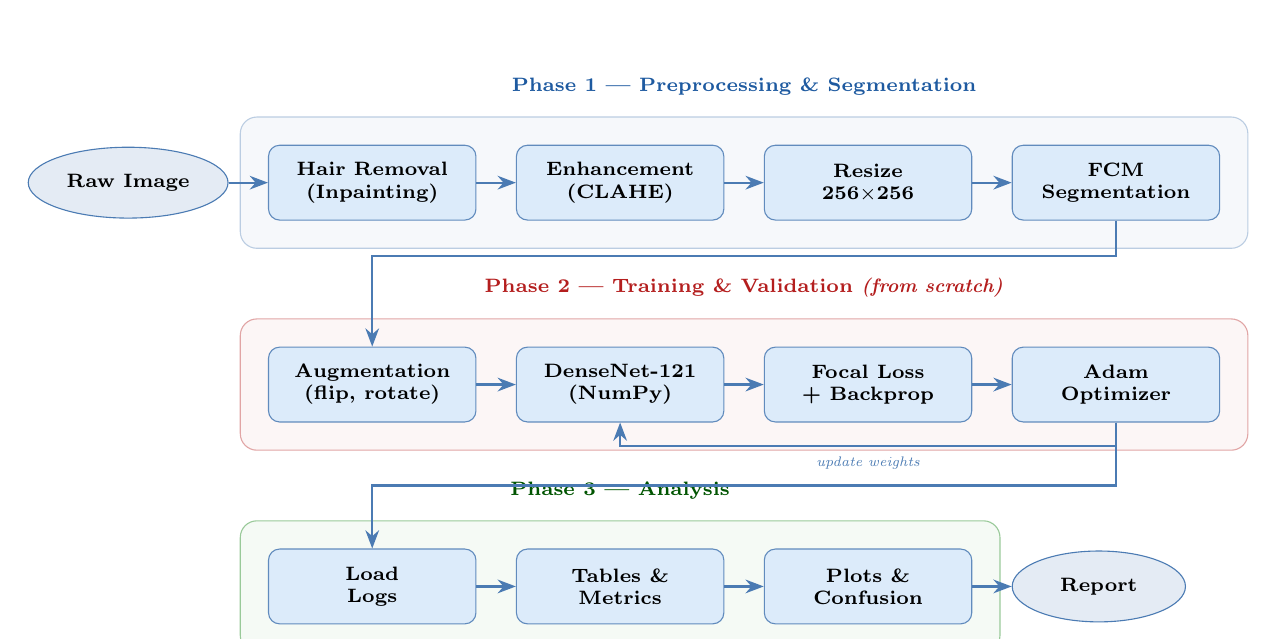
\begin{tikzpicture}[
    io/.style={ellipse, draw=mainblue!80, fill=mainblue!12,
               minimum width=2.2cm, minimum height=0.9cm,
               align=center, font=\scriptsize\bfseries},
    proc/.style={rectangle, rounded corners=4pt,
                 draw=mainblue!70, fill=lightblue,
                 minimum width=2.5cm, minimum height=0.95cm,
                 align=center, font=\scriptsize\bfseries,
                 text width=2.4cm},
    grp/.style={rectangle, rounded corners=6pt,
                draw=mainblue!30, fill=mainblue!4,
                inner sep=10pt},
    arr/.style={-Stealth, thick, mainblue!80},
    lbl/.style={font=\scriptsize\bfseries\color{mainblue}, above=4pt},
  ]

  %% ROW 1 -- Phase 1
  \node[io]   (img)    {Raw Image};
  \node[proc, right=0.5cm of img]   (hair)   {Hair Removal\\(Inpainting)};
  \node[proc, right=0.5cm of hair]  (enh)    {Enhancement\\(CLAHE)};
  \node[proc, right=0.5cm of enh]   (resize) {Resize\\256$\times$256};
  \node[proc, right=0.5cm of resize](fcm)    {FCM\\Segmentation};

  \begin{scope}[on background layer]
    \node[grp, fit=(hair)(enh)(resize)(fcm)] (ph1box) {};
  \end{scope}
  \node[lbl] at (ph1box.north) {Phase 1 --- Preprocessing \& Segmentation};

  \draw[arr] (img)--(hair);
  \draw[arr] (hair)--(enh);
  \draw[arr] (enh)--(resize);
  \draw[arr] (resize)--(fcm);

  %% ROW 2 -- Phase 2
  \node[proc, below=1.6cm of hair]  (aug)    {Augmentation\\(flip, rotate)};
  \node[proc, right=0.5cm of aug]   (dn)     {DenseNet-121\\(NumPy)};
  \node[proc, right=0.5cm of dn]    (focal)  {Focal Loss\\+ Backprop};
  \node[proc, right=0.5cm of focal] (adam)   {Adam\\Optimizer};

  \begin{scope}[on background layer]
    \node[grp, draw=codered!40, fill=codered!4,
          fit=(aug)(dn)(focal)(adam)] (ph2box) {};
  \end{scope}
  \node[font=\scriptsize\bfseries\color{codered}, above=4pt] at (ph2box.north)
    {Phase 2 --- Training \& Validation \textit{(from scratch)}};

  \draw[arr] (fcm.south) -- ++(0,-0.45) -| (aug.north);
  \draw[arr] (aug)--(dn);
  \draw[arr] (dn)--(focal);
  \draw[arr] (focal)--(adam);
  \draw[arr] (adam.south) -- ++(0,-0.3) -|
             node[near start, below, font=\tiny\itshape] {update weights}
             (dn.south);

  %% ROW 3 -- Phase 3
  \node[proc, below=1.6cm of aug]   (load)   {Load\\Logs};
  \node[proc, right=0.5cm of load]  (tabs)   {Tables \&\\Metrics};
  \node[proc, right=0.5cm of tabs]  (viz)    {Plots \&\\Confusion};
  \node[io,   right=0.5cm of viz]   (report) {Report};

  \begin{scope}[on background layer]
    \node[grp, draw=codegreen!40, fill=codegreen!4,
          fit=(load)(tabs)(viz)] (ph3box) {};
  \end{scope}
  \node[font=\scriptsize\bfseries\color{codegreen!70!black}, above=4pt] at (ph3box.north)
    {Phase 3 --- Analysis};

  \draw[arr] (adam.south) -- ++(0,-0.8) -| (load.north);
  \draw[arr] (load)--(tabs);
  \draw[arr] (tabs)--(viz);
  \draw[arr] (viz)--(report);

  \end{tikzpicture}
  \caption{End-to-end pipeline: from raw dermoscopy image to classification report}
  \label{fig:pipeline}
\end{figure}

% ==========================================================
\chapter{Project Directory Structure}
% ==========================================================

\section{Top-Level Layout}

The repository is organised into three main directories — one per pipeline phase — plus a shared results folder produced by Phase 1 that is consumed by Phase 2.

\begin{center}
\ttfamily\small
\begin{tabular}{@{}l@{}}
Deep Learning Project/\\
\quad|-- Dara Preprocessing \& Segmentation/\\
\quad|\quad\quad|-- src/\\
\quad|\quad\quad|\quad\quad`-- 01\_preprocessing\_and\_segmentation.ipynb\\
\quad|\quad\quad`-- results/\\
\quad|\quad\quad\quad\quad|-- ISIC2018\_Task3\_Training\_GroundTruth.csv\\
\quad|\quad\quad\quad\quad|-- ISIC2018\_Task3\_Test\_GroundTruth.csv\\
\quad|\quad\quad\quad\quad|-- images/training/\ \ (segmented training JPEGs)\\
\quad|\quad\quad\quad\quad`-- images/testing/\ \ \ (segmented test JPEGs)\\
\quad|\\
\quad|-- Training and Validation/\\
\quad|\quad\quad|-- train.py\\
\quad|\quad\quad|-- configs/config.yaml\\
\quad|\quad\quad|-- src/\\
\quad|\quad\quad|\quad\quad|-- dataset.py\\
\quad|\quad\quad|\quad\quad|-- model.py\\
\quad|\quad\quad|\quad\quad|-- losses.py\\
\quad|\quad\quad|\quad\quad|-- metrics.py\\
\quad|\quad\quad|\quad\quad|-- trainer.py\\
\quad|\quad\quad|\quad\quad`-- utils.py\\
\quad|\quad\quad`-- logs/\\
\quad|\quad\quad\quad\quad|-- metrics.csv\\
\quad|\quad\quad\quad\quad|-- best\_metrics.json\\
\quad|\quad\quad\quad\quad|-- best\_confusion\_matrix.npy\\
\quad|\quad\quad\quad\quad`-- train.log\\
\quad|\\
\quad`-- Analysis/\\
\quad\quad\quad\quad|-- analyze.py\\
\quad\quad\quad\quad|-- configs/analysis\_config.yaml\\
\quad\quad\quad\quad|-- src/\\
\quad\quad\quad\quad|\quad\quad|-- loader.py\\
\quad\quad\quad\quad|\quad\quad|-- tables.py\\
\quad\quad\quad\quad|\quad\quad`-- visualizer.py\\
\quad\quad\quad\quad`-- outputs/\ \ (PNG plots, CSV/MD tables)\\
\end{tabular}
\end{center}

\section{File Descriptions}

\subsection{Preprocessing \& Segmentation}

\begin{longtable}{>{\ttfamily\small}p{7.2cm} p{8cm}}
  \toprule
  \normalfont\textbf{File / Directory} & \textbf{Purpose} \\
  \midrule
  \endhead
  \bottomrule
  \endfoot
  src/01\_preprocessing\_and\_segmentation.ipynb
    & Jupyter notebook containing the full image-processing pipeline: hair removal, CLAHE enhancement, Black Hat / Gaussian filtering, adaptive thresholding, inpainting, and Fuzzy C-Means (FCM) segmentation. Produces the segmented JPEG images consumed by Phase 2. \\[4pt]
  results/ISIC2018\_Task3\_Training\-\_GroundTruth.csv
    & One-hot encoded ground-truth labels for the training set (columns: \texttt{image}, MEL, NV, BCC, AKIEC, BKL, DF, VASC). \\[4pt]
  results/ISIC2018\_Task3\_Test\-\_GroundTruth.csv
    & Same format for the validation / test set. \\[4pt]
  results/images/training/
    & Segmented training images (filename pattern: \texttt{ISIC\_XXXXXXX\_segmented.jpg}). \\[4pt]
  results/images/testing/
    & Segmented test images (filename pattern: \texttt{ISIC\_XXXXXXX\_Test\_Segmented.jpg}). \\
\end{longtable}

\subsection{Training and Validation}

\begin{longtable}{>{\ttfamily\small}p{4.2cm} p{11cm}}
  \toprule
  \normalfont\textbf{File} & \textbf{Purpose} \\
  \midrule
  \endhead
  \bottomrule
  \endfoot
  train.py
    & Entry point. Parses CLI arguments, loads the YAML config, seeds RNG, initialises the logger, device, dataloaders, model, loss, and optimizer, then calls \texttt{Trainer.fit()}. \\[4pt]
  configs/config.yaml
    & All hyper-parameters in one place: data paths, model settings, training schedule, augmentation probabilities, early-stopping criteria, and logging preferences. \\[4pt]
  src/dataset.py
    & \texttt{SkinLesionDataset}, \texttt{ImageTransform} (augmentation), and a custom \texttt{DataLoader} with weighted random sampling. \\[4pt]
  src/model.py
    & Complete DenseNet-121 architecture implemented with pure NumPy. Contains every layer from scratch: \texttt{Conv2D}, \texttt{BatchNorm2D}, \texttt{ReLU}, \texttt{Dropout}, \texttt{MaxPool2D}, \texttt{AvgPool2D}, \texttt{Linear}, \texttt{DenseLayer}, \texttt{DenseBlock}, \texttt{TransitionLayer}. \\[4pt]
  src/losses.py
    & \texttt{FocalLoss} — forward and analytic backward pass; \texttt{build\_loss} factory that optionally adds per-class alpha weights. \\[4pt]
  src/metrics.py
    & \texttt{compute\_all\_metrics} — computes per-class and macro Accuracy, Precision, Recall, Specificity, F1, Dice, Jaccard, and AUC-ROC from predictions and probabilities. \\[4pt]
  src/trainer.py
    & \texttt{Trainer} class: two-phase training loop (frozen backbone then full fine-tune), epoch-level validation, CSV logging, atomic model artifact saving, and early stopping. \\[4pt]
  src/utils.py
    & \texttt{AdamOptimizer}, \texttt{CosineAnnealingScheduler}, \texttt{ReduceOnPlateauScheduler}, \texttt{load\_config}, \texttt{set\_seed}, \texttt{setup\_logger}, \texttt{get\_device}. \\[4pt]
  logs/metrics.csv
    & Per-epoch training and validation metrics for the full run. \\[4pt]
  logs/best\_metrics.json
    & Full per-class and macro metrics snapshot at the epoch with the best macro F1. \\[4pt]
  logs/best\_confusion\_matrix.npy
    & NumPy binary of the confusion matrix at the best epoch. \\[4pt]
  logs/train.log
    & Full timestamped training log (DEBUG level). \\
\end{longtable}

\subsection{Analysis}

\begin{longtable}{>{\ttfamily\small}p{4.2cm} p{11cm}}
  \toprule
  \normalfont\textbf{File} & \textbf{Purpose} \\
  \midrule
  \endhead
  \bottomrule
  \endfoot
  analyze.py
    & Entry point. Loads training artifacts from the \texttt{Training and Validation/logs/} directory and orchestrates all tabulation and plotting steps. \\[4pt]
  configs/analysis\_config.yaml
    & Paths to the training logs and the output directory; decouples the analysis tool from the training directory layout. \\[4pt]
  src/loader.py
    & \texttt{load\_artifacts} — reads \texttt{metrics.csv}, \texttt{best\_metrics.json}, \texttt{final\_metrics.json}, and \texttt{best\_confusion\_matrix.npy}; returns them as a \texttt{SimpleNamespace}. \\[4pt]
  src/tables.py
    & \texttt{build\_per\_class\_table}, \texttt{macro\_summary\_table}, \texttt{best\_and\_worst\_classes}, \texttt{epoch\_history\_table} — export CSV and Markdown tables. \\[4pt]
  src/visualizer.py
    & \texttt{plot\_training\_curves}, \texttt{plot\_per\_class\_metrics\_bar}, \texttt{plot\_confusion\_matrix}, \texttt{plot\_per\_class\_metric\_comparison} — generate all PNG figures using Matplotlib and Seaborn. \\[4pt]
  outputs/
    & Contains all generated figures and tables (see Chapter~\ref{ch:results}). \\
\end{longtable}

% ==========================================================
\chapter{Phase 1: Data Preprocessing \& Segmentation}
% ==========================================================

\begin{notebox}[Attribution]
This phase was provided as part of the project framework and is not original work of the group. It is documented here for completeness and to explain the data format consumed by Phase~2.
\end{notebox}

\section{Overview}

The preprocessing notebook transforms raw dermoscopy JPEG images into clean, segmented lesion images that isolate the region of interest (ROI) from background skin and artefacts such as hair and air bubbles.

\section{Preprocessing Pipeline}

Figure~\ref{fig:preprocess} shows the sequential image-processing steps applied to each input image.

\begin{figure}[ht]
  \centering
  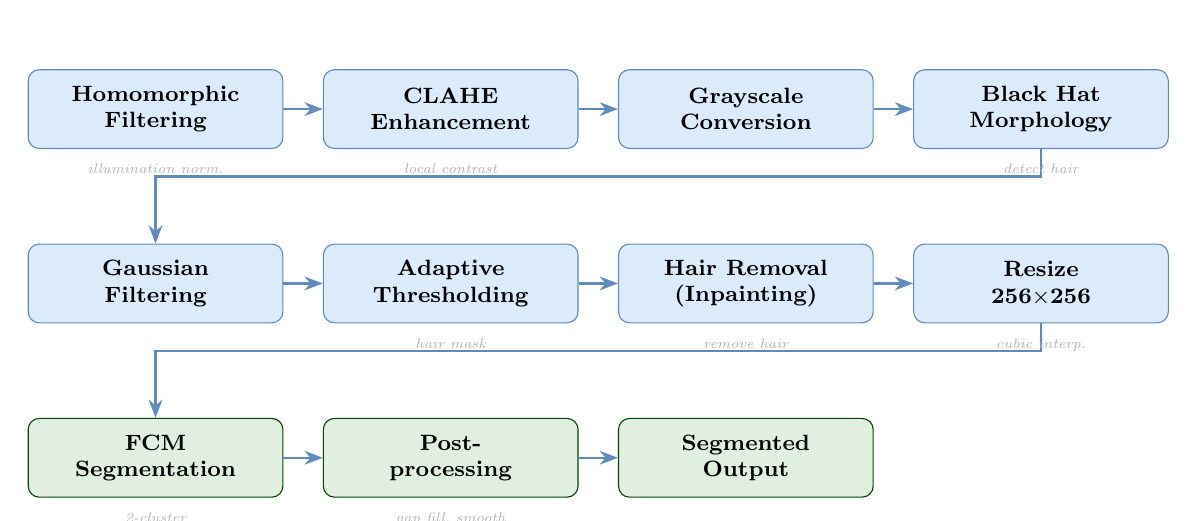
\begin{tikzpicture}[
    ppstep/.style={rectangle, rounded corners=4pt,
                 draw=mainblue!70, fill=lightblue,
                 minimum width=3.2cm, minimum height=1.0cm,
                 align=center, font=\footnotesize\bfseries,
                 text width=3.0cm},
    arr/.style={-Stealth, thick, mainblue!70},
    lbl/.style={font=\tiny\itshape, text=gray!60, below=2pt},
  ]
    \node[ppstep] (hom)  {Homomorphic\\Filtering};
    \node[ppstep, right=0.5cm of hom]  (clahe) {CLAHE\\Enhancement};
    \node[ppstep, right=0.5cm of clahe](gray)  {Grayscale\\Conversion};
    \node[ppstep, right=0.5cm of gray] (bhat)  {Black Hat\\Morphology};

    \node[ppstep, below=1.2cm of hom]  (gauss) {Gaussian\\Filtering};
    \node[ppstep, right=0.5cm of gauss](thresh){Adaptive\\Thresholding};
    \node[ppstep, right=0.5cm of thresh](inp)  {Hair Removal\\(Inpainting)};
    \node[ppstep, right=0.5cm of inp]  (res)   {Resize\\256$\times$256};

    \node[ppstep, below=1.2cm of gauss, fill=codegreen!12, draw=codegreen!60!black]
                                     (fcm)   {FCM\\Segmentation};
    \node[ppstep, right=0.5cm of fcm, fill=codegreen!12, draw=codegreen!60!black]
                                     (post)  {Post-\\processing};
    \node[ppstep, right=0.5cm of post, fill=codegreen!12, draw=codegreen!60!black]
                                     (out)   {Segmented\\Output};

    \draw[arr] (hom)--(clahe);
    \draw[arr] (clahe)--(gray);
    \draw[arr] (gray)--(bhat);
    \draw[arr] (bhat.south) -- ++(0,-0.35) -| (gauss.north);
    \draw[arr] (gauss)--(thresh);
    \draw[arr] (thresh)--(inp);
    \draw[arr] (inp)--(res);
    \draw[arr] (res.south) -- ++(0,-0.35) -| (fcm.north);
    \draw[arr] (fcm)--(post);
    \draw[arr] (post)--(out);

    \node[lbl] at (hom.south)   {illumination norm.};
    \node[lbl] at (clahe.south) {local contrast};
    \node[lbl] at (bhat.south)  {detect hair};
    \node[lbl] at (thresh.south){hair mask};
    \node[lbl] at (inp.south)   {remove hair};
    \node[lbl] at (res.south)   {cubic interp.};
    \node[lbl] at (fcm.south)   {2-cluster};
    \node[lbl] at (post.south)  {gap fill, smooth};
  \end{tikzpicture}
  \caption{Data preprocessing and segmentation pipeline}
  \label{fig:preprocess}
\end{figure}

\subsection{Step Descriptions}

\begin{description}[leftmargin=0pt, style=nextline]
  \item[Homomorphic Filtering]
    Normalises non-uniform illumination by separating and suppressing the low-frequency illumination component while preserving high-frequency reflectance detail. Operates in the log-frequency domain.

  \item[CLAHE (Contrast Limited Adaptive Histogram Equalization)]
    Applies local histogram equalisation with a clip limit to avoid noise amplification. Improves the visibility of fine lesion structures and colour gradients critical for segmentation.

  \item[Black Hat Morphological Filtering]
    Detects dark, elongated structures (hair fibres) against a brighter background by subtracting a morphologically closed image from the original. The resulting high-response regions form the hair detection mask.

  \item[Gaussian Filtering]
    Smooths the hair mask to reduce spurious detections before thresholding.

  \item[Adaptive Thresholding]
    Converts the smoothed hair response map into a binary hair mask, with the threshold adapting to local pixel neighbourhood statistics.

  \item[Inpainting (Hair Removal)]
    Uses the binary hair mask (dilated slightly to ensure full coverage) to fill over hair pixels using surrounding context, yielding a clean skin surface.

  \item[Resize to 256$\times$256]
    Standardises image dimensions using cubic interpolation (bicubic), which preserves edge sharpness better than bilinear at this scale.

  \item[Fuzzy C-Means (FCM) Segmentation]
    Groups image pixels into $k=2$ clusters (lesion ROI and background skin) using fuzzy membership. Parameters: fuzziness exponent $m = 0.001$, convergence tolerance $\varepsilon = 10^{-5}$, maximum 1{,}000 iterations. The ROI cluster forms the binary segmentation mask.

  \item[Post-processing]
    Fills small holes inside the segmentation mask (morphological closing) and smooths the mask boundary to remove jagged edges, improving the quality of the extracted region.
\end{description}

\section{Output Format}

Segmented images are saved as JPEG files with the naming conventions:
\begin{itemize}[nosep]
  \item \textbf{Training:} \texttt{ISIC\_XXXXXXX\_segmented.jpg}
  \item \textbf{Testing:} \texttt{ISIC\_XXXXXXX\_Test\_Segmented.jpg}
\end{itemize}
Ground-truth labels are stored as one-hot-encoded CSV files alongside the images. The classifier in Phase~2 reads both the images and CSV files directly.

% ==========================================================
\chapter{Phase 2: Training \& Validation (From Scratch)}
\label{ch:training}
% ==========================================================

This phase is the original contribution of the project. Every component — the model, the optimiser, the loss function, the data pipeline, and the training loop — was implemented using \textbf{pure NumPy with no deep learning library}.

\section{Configuration (\texttt{configs/config.yaml})}

All hyper-parameters are centralised in a YAML file and loaded into a \texttt{SimpleNamespace} hierarchy at startup. Key settings:

\begin{table}[ht]
  \centering
  \caption{Key training hyper-parameters}
  \label{tab:config}
  \begin{tabular}{lll}
    \toprule
    \textbf{Parameter} & \textbf{Value} & \textbf{Notes} \\
    \midrule
    Architecture        & DenseNet-121       & Built from scratch \\
    Input size          & 224$\times$224     & Resized from 256$\times$256 \\
    Dropout             & 0.6                & Heavy regularisation for small dataset \\
    Batch size          & 32                 & \\
    Phase-1 epochs      & 8                  & Frozen backbone, classifier head only \\
    Phase-1 LR          & $10^{-3}$          & High LR safe; only head updates \\
    Phase-2 LR          & $3\times10^{-5}$   & Low LR for full fine-tuning \\
    LR scheduler        & Cosine annealing   & Applied in Phase~2 \\
    Loss                & Focal ($\gamma=2$) & Addresses class imbalance \\
    Weight decay        & $10^{-3}$          & L2 regularisation \\
    Weighted sampler    & Enabled            & Over-samples minority classes \\
    Early stopping      & patience=12        & Monitors macro F1 \\
    Seed                & 42                 & \\
    \bottomrule
  \end{tabular}
\end{table}

\section{Data Pipeline (\texttt{src/dataset.py})}

\subsection{\texttt{load\_and\_clean\_csv}}
Reads a ground-truth CSV, verifies that every referenced image file exists on disk, and derives an integer \texttt{label} column from the one-hot columns via \texttt{argmax}.

\subsection{\texttt{ImageTransform}}

Applies a configurable augmentation and normalisation pipeline. The transform is implemented as a callable class:

\begin{lstlisting}[caption={Core transform call --- augmentation and normalisation},label={lst:transform}]
def __call__(self, pil_img: Image.Image) -> np.ndarray:
    pil_img = pil_img.resize((self.size, self.size), Image.BILINEAR)
    if self.augment and self.aug is not None:
        pil_img = self._rotate(pil_img, self.aug.rotation_deg)
    img = np.array(pil_img, dtype=np.float32) / 255.0
    if self.augment and self.aug is not None:
        img = self._hflip(img, self.aug.horizontal_flip)
        img = self._vflip(img, self.aug.vertical_flip)
        img = self._color_jitter(img, self.aug.color_jitter)
    img = (img - self.MEAN) / self.STD   # ImageNet normalisation
    return img.transpose(2, 0, 1).astype(np.float32)  # HWC -> CHW
\end{lstlisting}

Training augmentations applied: random horizontal flip (p=0.5), vertical flip (p=0.5), rotation up to $\pm30°$, and colour jitter (brightness, contrast, saturation, factor=0.2). Validation uses only resize and normalise.

\subsection{\texttt{DataLoader} with Weighted Sampling}

A custom \texttt{DataLoader} iterates over the dataset in batches. When \texttt{use\_weighted\_sampler} is enabled, each epoch samples indices \textit{with replacement} using per-sample weights inversely proportional to class frequency:

\[
  w_i = \frac{1}{\text{count}(\text{class of sample } i)}
\]

This effectively over-samples minority classes (DF, VASC) and under-samples the dominant class (NV), producing balanced mini-batches without discarding data.

\section{Model Architecture (\texttt{src/model.py})}

\subsection{Low-Level Primitives}

\subsubsection{\texttt{\_im2col} / \texttt{\_col2im}}

Convolution is implemented via the \emph{im2col} technique, which reshapes the input tensor into a 2-D matrix so that each convolution window becomes a row. The matrix product $\mathbf{W}_{\text{col}} \cdot \mathbf{X}_{\text{col}}^{\top}$ then computes all spatial positions simultaneously:

\begin{lstlisting}[caption={im2col using NumPy stride tricks},label={lst:im2col}]
def _im2col(x, kernel_size, stride, padding):
    N, C, H, W = x.shape
    H_out = (H + 2*padding - kernel_size) // stride + 1
    W_out = (W + 2*padding - kernel_size) // stride + 1
    x_pad = np.pad(x, ((0,0),(0,0),(padding,padding),(padding,padding)))
    s0, s1, s2, s3 = x_pad.strides
    col = np.lib.stride_tricks.as_strided(
        x_pad,
        shape=(N, C, kernel_size, kernel_size, H_out, W_out),
        strides=(s0, s1, s2, s3, s2*stride, s3*stride),
    )
    return col.transpose(0,4,5,1,2,3).reshape(N*H_out*W_out, -1).copy(), H_out, W_out
\end{lstlisting}

The gradient \texttt{\_col2im} is the transpose operation, scattering gradient contributions back to each input position.

\subsubsection{Layer Base Class}

All layers inherit from a common \texttt{Layer} interface exposing \texttt{forward}, \texttt{backward}, \texttt{parameters}, \texttt{gradients}, and a \texttt{frozen} flag for selective gradient blocking.

\subsection{Individual Layers}

\begin{description}[leftmargin=0pt, style=nextline]
  \item[\texttt{Conv2D}]
    Stores weight tensor $\mathbf{W} \in \mathbb{R}^{C_{\text{out}} \times C_{\text{in}} \times k \times k}$ initialised with He initialisation. Forward: \texttt{im2col} + matrix multiply. Backward: weight gradient from outer product of gradient and cached column matrix; input gradient via \texttt{col2im}.

  \item[\texttt{BatchNorm2D}]
    Maintains running mean and variance for inference. During training, normalises over the $(N, H, W)$ dimensions and scales by learned $\gamma$, $\beta$. Analytic backward computes $\partial L/\partial x$ via the chain rule through mean and variance.

  \item[\texttt{ReLU}]
    Caches a Boolean mask $(\mathbf{x} > 0)$ during forward; gates the gradient in backward.

  \item[\texttt{Dropout}]
    Inverted dropout: scales the random binary mask by $1/(1-p)$ so the expected output magnitude is unchanged at test time. Disabled automatically when \texttt{training=False}.

  \item[\texttt{MaxPool2D} / \texttt{AvgPool2D}]
    Both use \texttt{im2col}. \texttt{MaxPool2D} caches the argmax index per pool window for gradient routing. \texttt{AvgPool2D} spreads the gradient uniformly across all positions.

  \item[\texttt{Linear}]
    Standard fully connected layer: $\mathbf{y} = \mathbf{x}\mathbf{W}^{\top} + \mathbf{b}$.
\end{description}

\subsection{DenseNet Building Blocks}

Figure~\ref{fig:densenet} shows the DenseNet-121 macro-architecture.

\begin{figure}[ht]
  \centering
  \scalebox{0.62}{%
  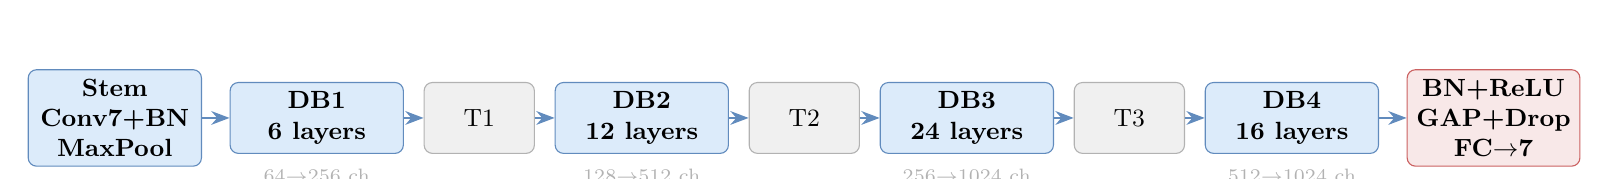
\begin{tikzpicture}[
    blk/.style={rectangle, rounded corners=3pt,
                draw=mainblue!70, fill=lightblue,
                minimum width=2.2cm, minimum height=0.9cm,
                align=center, font=\small\bfseries},
    trans/.style={rectangle, rounded corners=3pt,
                  draw=gray!60, fill=gray!12,
                  minimum width=1.4cm, minimum height=0.9cm,
                  align=center, font=\small},
    head/.style={rectangle, rounded corners=3pt,
                 draw=codered!70, fill=codered!10,
                 minimum width=1.8cm, minimum height=0.9cm,
                 align=center, font=\small\bfseries},
    arr/.style={-Stealth, thick, mainblue!70},
    lbl/.style={font=\scriptsize, text=gray!60, below=2pt},
  ]
    \node[blk] (init) {Stem\\Conv7+BN\\MaxPool};
    \node[blk, right=0.35cm of init] (d1) {DB1\\6 layers};
    \node[trans, right=0.25cm of d1]  (t1) {T1};
    \node[blk, right=0.25cm of t1]   (d2) {DB2\\12 layers};
    \node[trans, right=0.25cm of d2]  (t2) {T2};
    \node[blk, right=0.25cm of t2]   (d3) {DB3\\24 layers};
    \node[trans, right=0.25cm of d3]  (t3) {T3};
    \node[blk, right=0.25cm of t3]   (d4) {DB4\\16 layers};
    \node[head, right=0.35cm of d4]   (cls){BN+ReLU\\GAP+Drop\\FC$\to$7};

    \draw[arr] (init)--(d1);
    \draw[arr] (d1)--(t1);
    \draw[arr] (t1)--(d2);
    \draw[arr] (d2)--(t2);
    \draw[arr] (t2)--(d3);
    \draw[arr] (d3)--(t3);
    \draw[arr] (t3)--(d4);
    \draw[arr] (d4)--(cls);

    \node[lbl] at (d1.south) {64$\to$256 ch};
    \node[lbl] at (d2.south) {128$\to$512 ch};
    \node[lbl] at (d3.south) {256$\to$1024 ch};
    \node[lbl] at (d4.south) {512$\to$1024 ch};
  \end{tikzpicture}}
  \caption{DenseNet-121 macro-architecture (from scratch, NumPy). DB=Dense Block, T=Transition, GAP=Global Avg Pool.}
  \label{fig:densenet}
\end{figure}

\subsubsection{\texttt{DenseLayer}}

Each dense layer implements the \emph{bottleneck} design: BN$\to$ReLU$\to$Conv(1$\times$1, $4k$ filters)$\to$BN$\to$ReLU$\to$Conv(3$\times$3, $k$ filters), where $k=32$ is the growth rate. The output is \emph{concatenated} with the input along the channel axis, creating a direct gradient path to all preceding layers:

\[
  \mathbf{x}_\ell = [\mathbf{x}_0, \mathbf{x}_1, \ldots, \mathbf{x}_{\ell-1}]
\]

\subsubsection{\texttt{DenseBlock}}

Stacks $n$ \texttt{DenseLayer} objects sequentially. After $n$ layers, the output has $C_{\text{in}} + n \cdot k$ channels. Backward pass reverses the layer order.

\subsubsection{\texttt{TransitionLayer}}

Between dense blocks, a transition layer performs BN$\to$ReLU$\to$Conv(1$\times$1, compression=$0.5$)$\to$AvgPool(2$\times$2) to halve spatial dimensions and reduce channel count.

\subsubsection{\texttt{DenseNet121} Top-Level Class}

\begin{itemize}[nosep]
  \item \textbf{Stem:} Conv(7$\times$7, 64, stride=2) + BN + ReLU + MaxPool(3$\times$3, stride=2).
  \item \textbf{Body:} 4 Dense Blocks with 6, 12, 24, 16 layers respectively, interleaved with 3 Transition Layers.
  \item \textbf{Head:} Final BN + ReLU + Global Average Pooling + Dropout(0.6) + Linear($\to$7).
  \item \textbf{Backbone freeze / unfreeze:} Sets \texttt{frozen=True} on all layers except the final \texttt{Linear} to enable Phase-1 training.
  \item \textbf{Persistence:} \texttt{save(path)} and \texttt{load(path)} serialise / deserialise all weight arrays via \texttt{np.savez} keyed by layer name.
\end{itemize}

\section{Loss Function (\texttt{src/losses.py})}

\subsection{Focal Loss}

Standard cross-entropy treats all samples equally. For heavily imbalanced datasets, easy majority-class samples dominate the gradient signal. Focal Loss addresses this by down-weighting well-classified examples:

\[
  \mathcal{L}_{\text{focal}} = -\alpha_t \bigl(1 - p_t\bigr)^{\gamma} \log p_t
\]

where $p_t$ is the model's predicted probability for the true class, $\gamma=2$ is the focusing parameter, and $\alpha_t$ is a per-class weight inversely proportional to class frequency.

The analytic backward pass computes:
\[
  \frac{\partial \mathcal{L}}{\partial z_j} =
  (1-p_t)^{\gamma}\bigl(p_j - \mathbf{1}_{j=t}\bigr)
  - \gamma(1-p_t)^{\gamma-1} p_t \log(p_t)\, \mathbf{1}_{j=t}
\]

where $z_j$ are the logits and $p_j = \text{softmax}(z)_j$.

\subsection{\texttt{build\_loss}}

Factory function that reads the config to decide whether to use Focal Loss or weighted cross-entropy (Focal with $\gamma=0$), and whether to use per-class $\alpha$ weights. When \texttt{use\_weighted\_sampler=True}, the sampler already balances batches so $\alpha$ is omitted.

\section{Metrics (\texttt{src/metrics.py})}

\texttt{compute\_all\_metrics} accepts ground-truth labels, predicted labels, and predicted probabilities, then returns:

\begin{itemize}[nosep]
  \item \textbf{Per-class:} Accuracy, Precision, Recall, Specificity, F1 (= Dice), Jaccard Index, AUC-ROC
  \item \textbf{Macro averages} across all seven classes
  \item \textbf{Confusion matrix}
\end{itemize}

AUC-ROC is computed from scratch using a trapezoid integration over the sorted score ranking for each class in a one-vs-rest fashion.

\section{Trainer (\texttt{src/trainer.py})}

\subsection{Two-Phase Training}

\begin{figure}[ht]
  \centering
  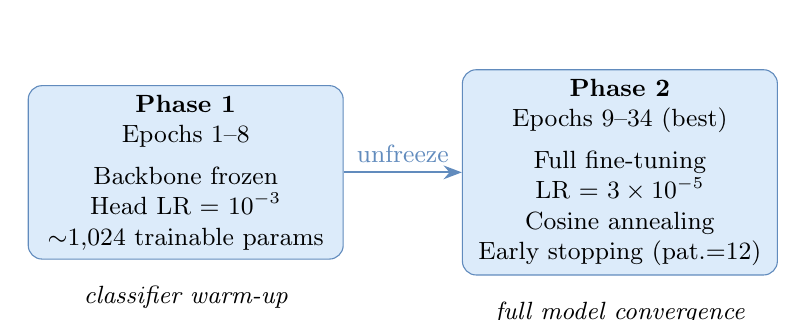
\begin{tikzpicture}[
    phase/.style={rectangle, rounded corners=5pt,
                  draw=mainblue!70, fill=lightblue,
                  minimum width=4cm, minimum height=2.2cm,
                  align=center, font=\small},
    arr/.style={-Stealth, thick, mainblue!70},
  ]
    \node[phase] (p1) {%
      \textbf{Phase 1}\\
      \small Epochs 1--8\\[4pt]
      Backbone frozen\\
      Head LR = $10^{-3}$\\
      $\sim$1{,}024 trainable params};
    \node[phase, right=1.5cm of p1] (p2) {%
      \textbf{Phase 2}\\
      \small Epochs 9--34 (best)\\[4pt]
      Full fine-tuning\\
      LR = $3\times10^{-5}$\\
      Cosine annealing\\
      Early stopping (pat.=12)};
    \draw[arr] (p1) -- node[above, font=\small]{unfreeze} (p2);
    \node[font=\small\itshape, below=6pt] at (p1.south) {classifier warm-up};
    \node[font=\small\itshape, below=6pt] at (p2.south) {full model convergence};
  \end{tikzpicture}
  \caption{Two-phase training strategy}
  \label{fig:twophase}
\end{figure}

\textbf{Phase 1} warms up the randomly initialised classifier head while keeping all convolution and batch-norm weights frozen. This prevents the random head from corrupting the backbone representations during early high-loss iterations.

\textbf{Phase 2} unfreezes the entire model and fine-tunes with a much lower learning rate under cosine annealing, allowing all layers to specialise for the skin-lesion domain.

\subsection{Key Methods}

\begin{description}[leftmargin=0pt, style=nextline]
  \item[\texttt{train\_one\_epoch}]
    Iterates over all training batches, runs forward/backward through the model and loss, and calls \texttt{optimizer.step(grads)}. Uses a \texttt{tqdm} progress bar with live loss display.

  \item[\texttt{validate}]
    Sets the model to eval mode (disables dropout and uses running statistics for BN), collects all predictions and probabilities, then calls \texttt{compute\_all\_metrics} and logs the results table.

  \item[\texttt{\_atomic\_save}]
    Writes artifacts to a temporary file and atomically renames it, guaranteeing that a partial write never overwrites a valid checkpoint.

  \item[\texttt{fit}]
    Outer training loop. Orchestrates phase transitions, calls \texttt{train\_one\_epoch} and \texttt{validate} each epoch, logs to CSV, checks early stopping, and saves best/final artifacts.
\end{description}

\section{Utilities (\texttt{src/utils.py})}

\subsection{Adam Optimizer}

Implements Adam with bias-corrected moment estimates:

\[
  \hat{m}_t = \frac{\beta_1 m_{t-1} + (1-\beta_1)g_t}{1-\beta_1^t}, \quad
  \hat{v}_t = \frac{\beta_2 v_{t-1} + (1-\beta_2)g_t^2}{1-\beta_2^t}
\]
\[
  \theta_t = \theta_{t-1} - \alpha \frac{\hat{m}_t}{\sqrt{\hat{v}_t}+\epsilon}
\]

Default values: $\beta_1=0.9$, $\beta_2=0.999$, $\epsilon=10^{-8}$. Optional L2 weight decay is applied to the raw gradient before moment accumulation.

\subsection{Cosine Annealing Scheduler}

Decays the learning rate from its initial value $\eta_{\max}$ to $\eta_{\min}=10^{-7}$ over $T_{\max}$ epochs:

\[
  \eta_t = \eta_{\min} + \frac{1}{2}(\eta_{\max} - \eta_{\min})
           \left(1 + \cos\!\left(\frac{\pi t}{T_{\max}}\right)\right)
\]

\subsection{Other Utilities}

\begin{itemize}[nosep]
  \item \texttt{load\_config}: YAML $\to$ nested \texttt{SimpleNamespace} for attribute-style access.
  \item \texttt{set\_seed}: Seeds both \texttt{random} and \texttt{numpy.random} for reproducibility.
  \item \texttt{setup\_logger}: Creates a dual-handler logger (file at DEBUG level, console at INFO level) with ISO timestamp formatting.
\end{itemize}

\section{Training Entry Point (\texttt{train.py})}

\texttt{main()} wires all components together. The diagram in Figure~\ref{fig:entrypoint} summarises the startup sequence.

\begin{figure}[ht]
  \centering
  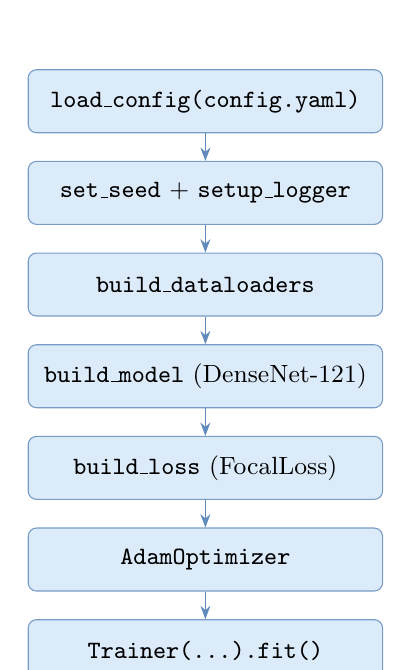
\begin{tikzpicture}[
    pstep/.style={rectangle, draw=mainblue!60, fill=lightblue,
                 rounded corners=3pt, minimum width=4.5cm,
                 minimum height=0.8cm, align=center, font=\small},
    arr/.style={-Stealth, mainblue!70},
  ]
    \node[pstep] (cfg)   {\texttt{load\_config(config.yaml)}};
    \node[pstep, below=0.35cm of cfg]  (seed)  {\texttt{set\_seed} + \texttt{setup\_logger}};
    \node[pstep, below=0.35cm of seed] (data)  {\texttt{build\_dataloaders}};
    \node[pstep, below=0.35cm of data] (model) {\texttt{build\_model} (DenseNet-121)};
    \node[pstep, below=0.35cm of model](loss)  {\texttt{build\_loss} (FocalLoss)};
    \node[pstep, below=0.35cm of loss] (opt)   {\texttt{AdamOptimizer}};
    \node[pstep, below=0.35cm of opt]  (train) {\texttt{Trainer(...).fit()}};

    \draw[arr] (cfg)--(seed);
    \draw[arr] (seed)--(data);
    \draw[arr] (data)--(model);
    \draw[arr] (model)--(loss);
    \draw[arr] (loss)--(opt);
    \draw[arr] (opt)--(train);
  \end{tikzpicture}
  \caption{Startup sequence in \texttt{train.py}}
  \label{fig:entrypoint}
\end{figure}

% ==========================================================
\chapter{Phase 3: Analysis}
% ==========================================================

After training completes, the \texttt{Analysis/} module reads the saved log artifacts and produces all evaluation tables and figures without re-running inference.

\section{Entry Point (\texttt{analyze.py})}

Loads the YAML config, reads all artifacts via \texttt{loader.load\_artifacts}, then calls:

\begin{enumerate}[nosep]
  \item \texttt{build\_per\_class\_table} — per-class metrics CSV and Markdown
  \item \texttt{macro\_summary\_table} — macro-averaged metrics CSV
  \item \texttt{best\_and\_worst\_classes} — ranked class summary text file
  \item \texttt{epoch\_history\_table} — copy of \texttt{metrics.csv} to outputs
  \item \texttt{plot\_training\_curves} — loss and metric curves
  \item \texttt{plot\_per\_class\_metrics\_bar} — 8-panel bar chart
  \item \texttt{plot\_confusion\_matrix} — count and normalised heatmaps
  \item \texttt{plot\_per\_class\_metric\_comparison} — per-metric comparison with best/worst highlighting
\end{enumerate}

\section{Key Functions}

\subsection{\texttt{load\_artifacts} (\texttt{src/loader.py})}

Validates that all required artifact paths exist before loading, raising a descriptive \texttt{FileNotFoundError} if training logs are absent. Returns a \texttt{SimpleNamespace} with fields \texttt{history} (DataFrame), \texttt{best} and \texttt{final} (dicts), and \texttt{confusion} (NumPy array).

\subsection{\texttt{build\_per\_class\_table} (\texttt{src/tables.py})}

Iterates over class names and metric keys, building a \texttt{pandas.DataFrame} that is saved as both a CSV and a Markdown table.

\subsection{\texttt{plot\_training\_curves} (\texttt{src/visualizer.py})}

Generates two figures:
\begin{itemize}[nosep]
  \item Training loss vs.\ validation loss over all epochs.
  \item Macro F1, Accuracy, AUC-ROC, and Recall over all epochs.
\end{itemize}

\subsection{\texttt{plot\_confusion\_matrix} (\texttt{src/visualizer.py})}

Produces two heatmaps from the saved \texttt{.npy} confusion matrix:
\begin{itemize}[nosep]
  \item \textbf{Count matrix:} raw prediction counts.
  \item \textbf{Normalised matrix:} row-normalised by true class totals (recall per cell).
\end{itemize}

\subsection{\texttt{plot\_per\_class\_metric\_comparison} (\texttt{src/visualizer.py})}

Creates an 8-panel figure (one panel per metric). Within each panel, the best-performing class bar is coloured green and the worst red, making performance outliers immediately apparent.

% ==========================================================
\chapter{Results and Evaluation}
\label{ch:results}
% ==========================================================

\section{Training Dynamics}

Figure~\ref{fig:loss} shows the training and validation loss curves across all epochs. The phase transition at epoch 8 is visible as a brief spike in validation loss before the model begins to fully fine-tune.

\begin{figure}[ht]
  \centering
  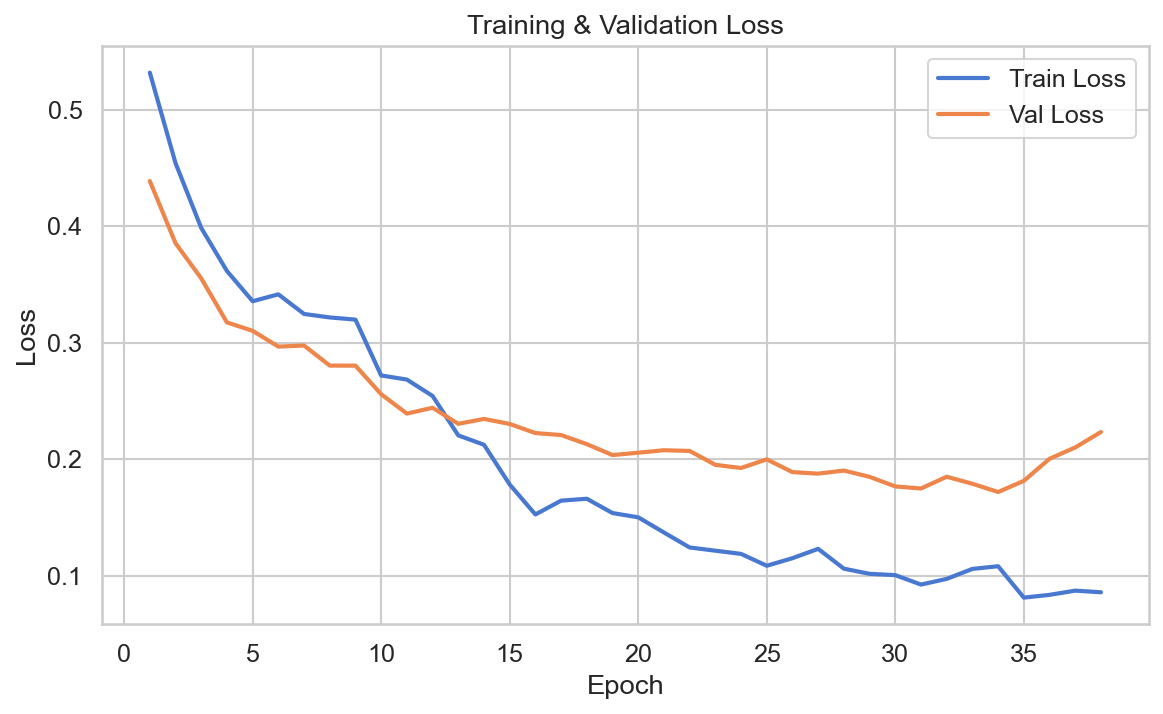
\includegraphics[width=0.85\textwidth]{training_loss_curves.png}
  \caption{Training and validation loss over epochs}
  \label{fig:loss}
\end{figure}

Figure~\ref{fig:metrics} shows the evolution of macro F1, Accuracy, AUC-ROC, and Recall on the validation set. The model converges to its best performance at \textbf{epoch 34}, after which early stopping terminates training.

\begin{figure}[ht]
  \centering
  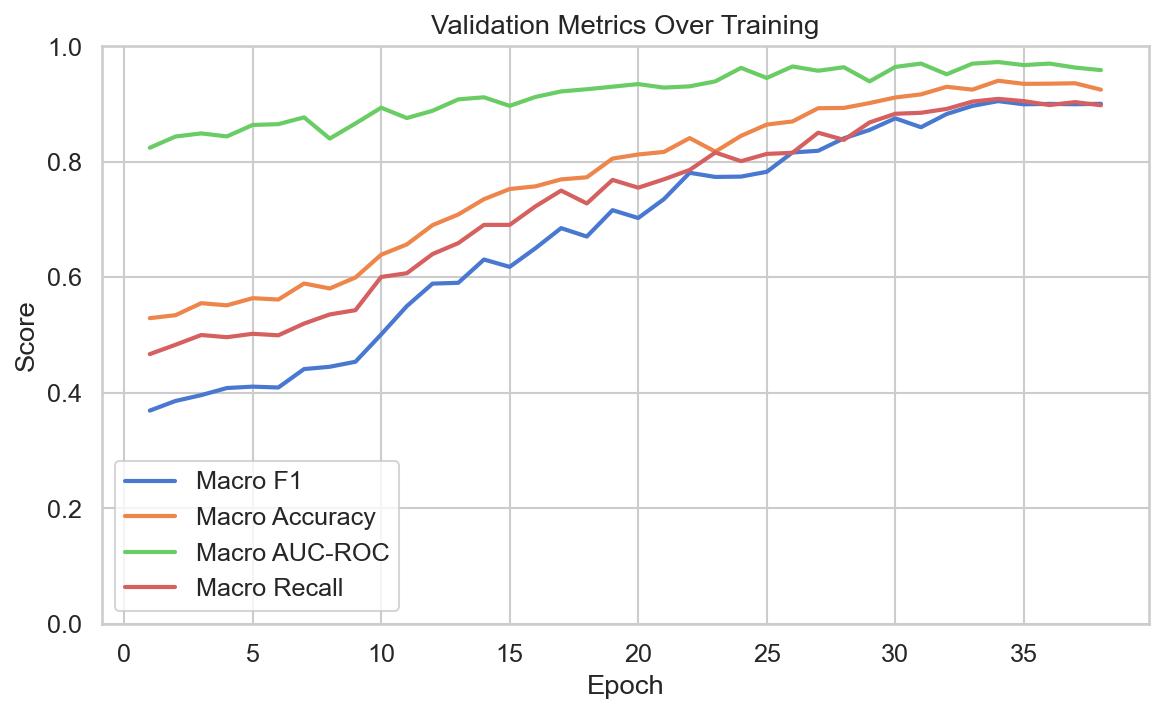
\includegraphics[width=0.85\textwidth]{training_metric_curves.png}
  \caption{Validation metric curves over epochs (macro averages)}
  \label{fig:metrics}
\end{figure}

\section{Final Performance}

Table~\ref{tab:macro} summarises the macro-averaged metrics at the best epoch.

\begin{table}[ht]
  \centering
  \caption{Macro-averaged metrics at best epoch (epoch 34)}
  \label{tab:macro}
  \begin{tabular}{lccccccc}
    \toprule
    \textbf{Accuracy} & \textbf{Precision} & \textbf{Recall} & \textbf{Specificity}
    & \textbf{F1} & \textbf{Dice} & \textbf{Jaccard} & \textbf{AUC-ROC} \\
    \midrule
    0.9405 & 0.9016 & 0.9091 & 0.9877 & 0.9052 & 0.9052 & 0.8283 & 0.9729 \\
    \bottomrule
  \end{tabular}
\end{table}

\section{Per-Class Performance}

Table~\ref{tab:perclass} shows the full per-class breakdown. NV achieves the highest F1 (0.9732), reflecting its dominance in the training set even after rebalancing. DF achieves the lowest F1 (0.8769), consistent with it being the rarest class.

\begin{table}[ht]
  \centering
  \caption{Per-class metrics at best epoch}
  \label{tab:perclass}
  \begin{tabular}{lcccccccc}
    \toprule
    \textbf{Class} & \textbf{Acc} & \textbf{Prec} & \textbf{Rec} & \textbf{Spec}
    & \textbf{F1} & \textbf{Dice} & \textbf{Jacc} & \textbf{AUC} \\
    \midrule
    MEL   & 0.9841 & 0.8991 & 0.8829 & 0.9921 & 0.8909 & 0.8909 & 0.8033 & 0.9681 \\
    NV    & 0.9689 & 0.9727 & 0.9738 & 0.9621 & 0.9732 & 0.9732 & 0.9479 & 0.9820 \\
    BCC   & 0.9881 & 0.9048 & 0.9223 & 0.9929 & 0.9135 & 0.9135 & 0.8407 & 0.9754 \\
    AKIEC & 0.9835 & 0.8738 & 0.8824 & 0.9908 & 0.8780 & 0.8780 & 0.7826 & 0.9612 \\
    BKL   & 0.9709 & 0.9087 & 0.8924 & 0.9845 & 0.9005 & 0.9005 & 0.8189 & 0.9643 \\
    DF    & 0.9894 & 0.8769 & 0.8769 & 0.9945 & 0.8769 & 0.8769 & 0.7808 & 0.9701 \\
    VASC  & 0.9960 & 0.8750 & 0.9333 & 0.9973 & 0.9032 & 0.9032 & 0.8235 & 0.9889 \\
    \midrule
    \textbf{Macro} & \textbf{0.9405} & \textbf{0.9016} & \textbf{0.9091} & \textbf{0.9877}
    & \textbf{0.9052} & \textbf{0.9052} & \textbf{0.8283} & \textbf{0.9729} \\
    \bottomrule
  \end{tabular}
\end{table}

\section{Confusion Matrix}

Figure~\ref{fig:cm} shows the normalised confusion matrix at the best epoch. The diagonal is uniformly high, indicating strong class separation. Minor confusion occurs between visually similar classes (MEL/NV and BKL/AKIEC).

\begin{figure}[ht]
  \centering
  \begin{subfigure}[b]{0.48\textwidth}
    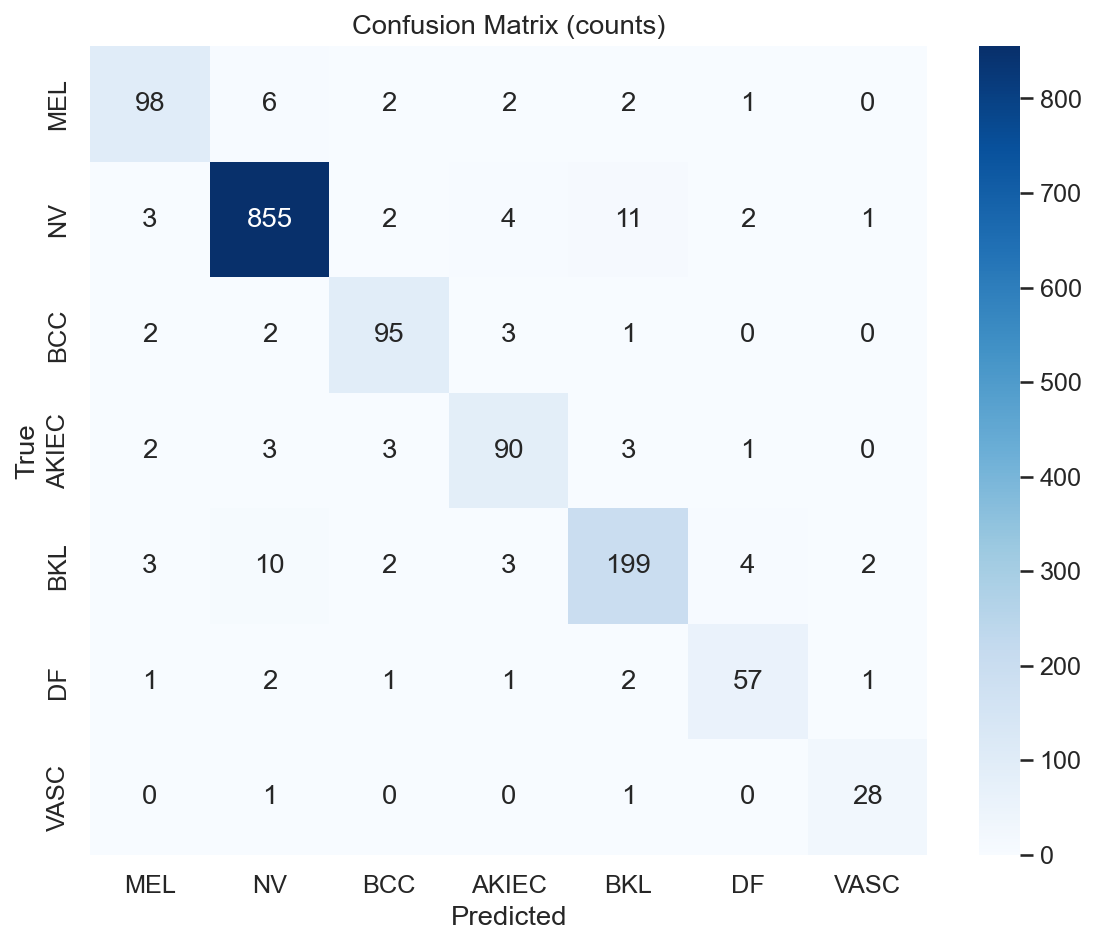
\includegraphics[width=\textwidth]{confusion_matrix_counts.png}
    \caption{Count confusion matrix}
  \end{subfigure}
  \hfill
  \begin{subfigure}[b]{0.48\textwidth}
    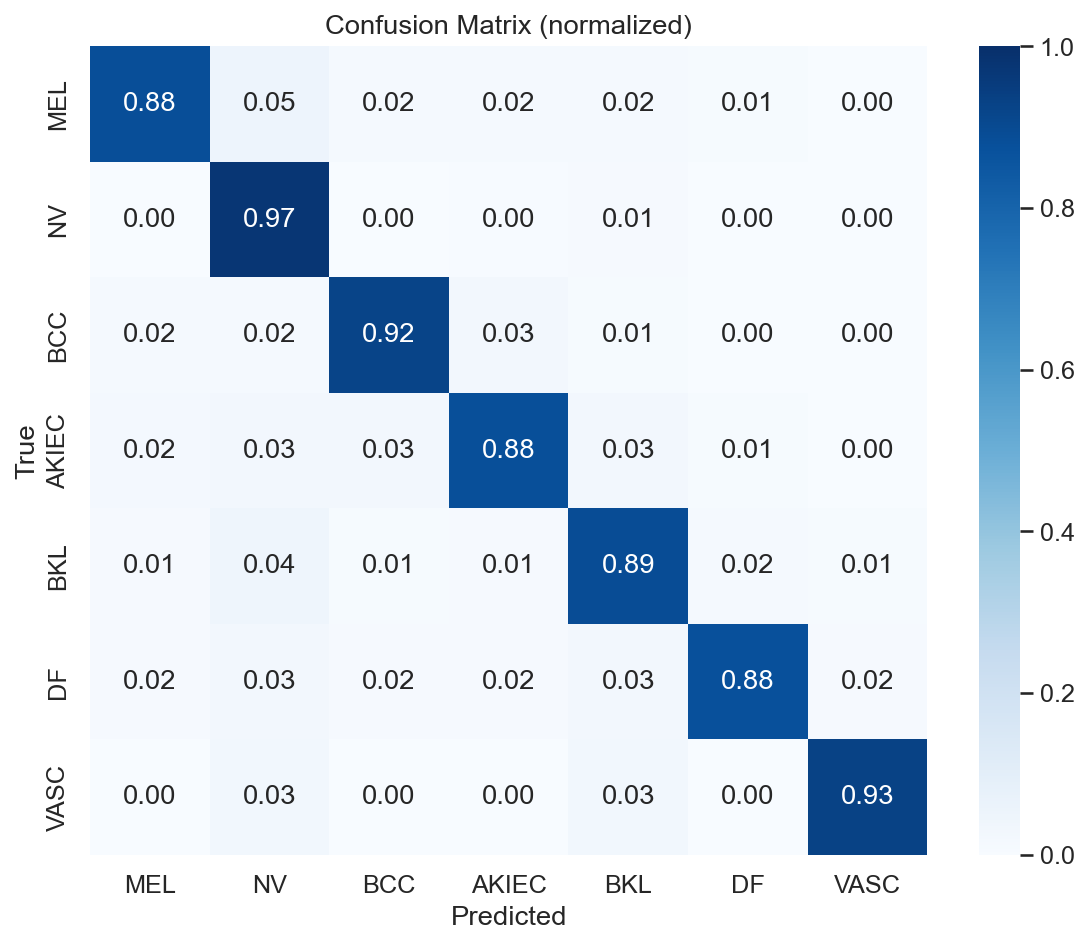
\includegraphics[width=\textwidth]{confusion_matrix_normalized.png}
    \caption{Normalised confusion matrix}
  \end{subfigure}
  \caption{Confusion matrices at best epoch (epoch 34)}
  \label{fig:cm}
\end{figure}

\section{Per-Class Metric Charts}

Figure~\ref{fig:bars} shows all eight metrics per class as grouped bar charts, and Figure~\ref{fig:comp} highlights the best (green) and worst (red) class for each metric.

\begin{figure}[ht]
  \centering
  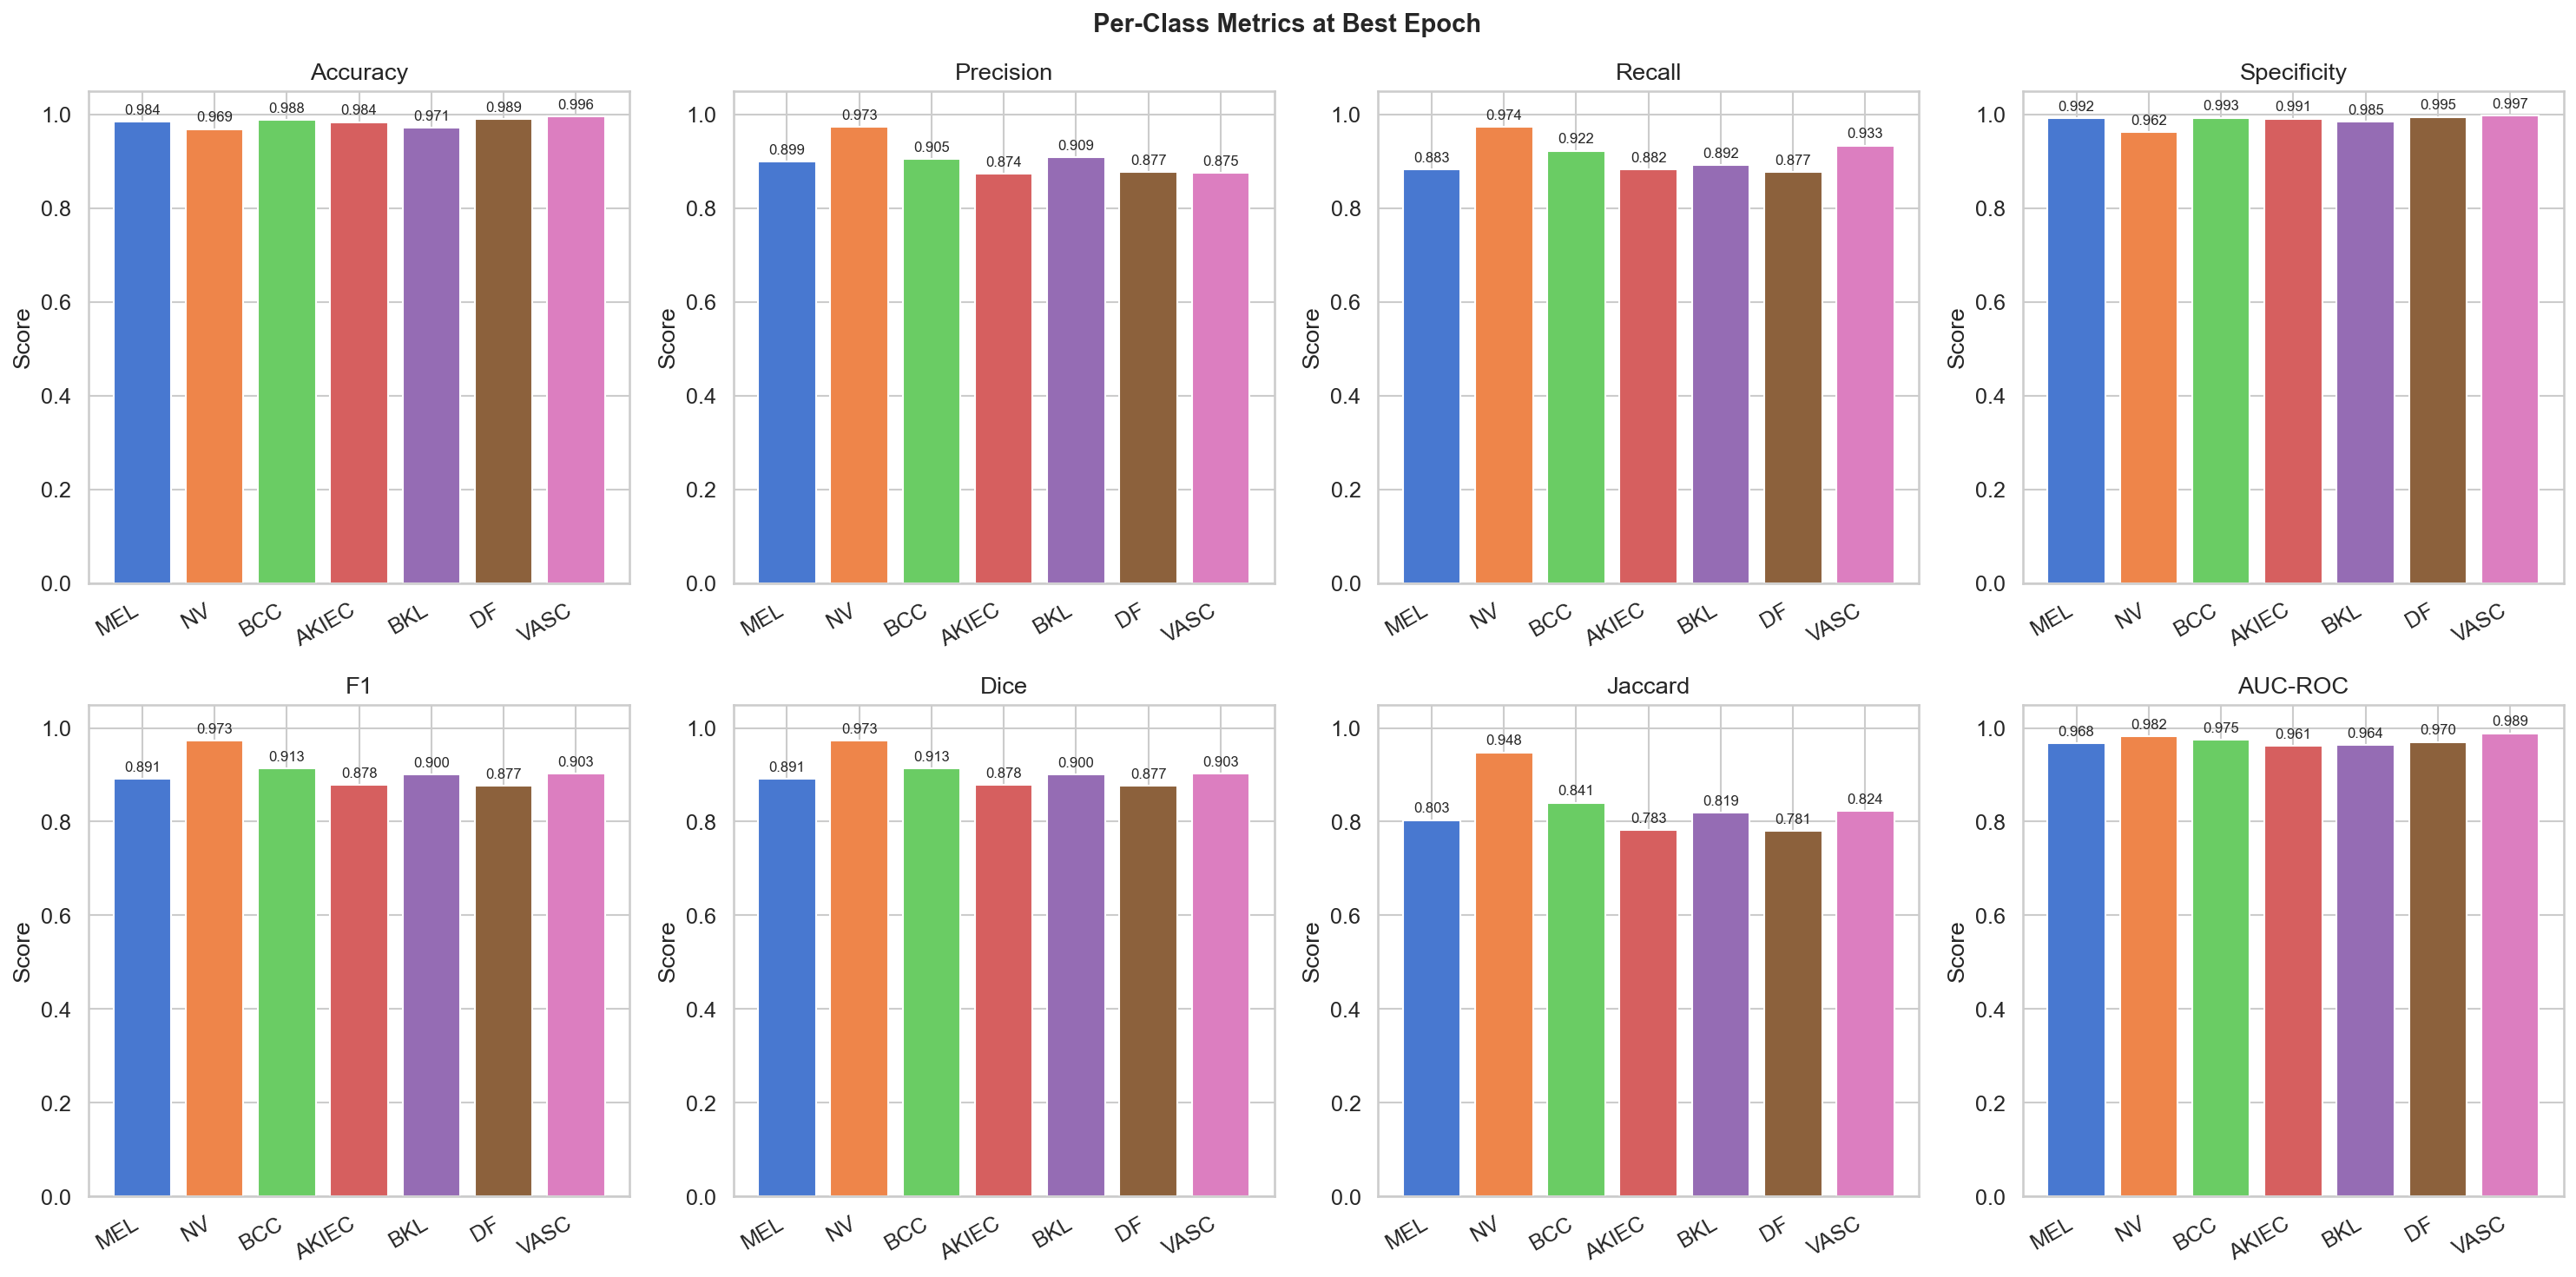
\includegraphics[width=\textwidth]{per_class_bars.png}
  \caption{Per-class metrics at best epoch (all eight metrics)}
  \label{fig:bars}
\end{figure}

\begin{figure}[ht]
  \centering
  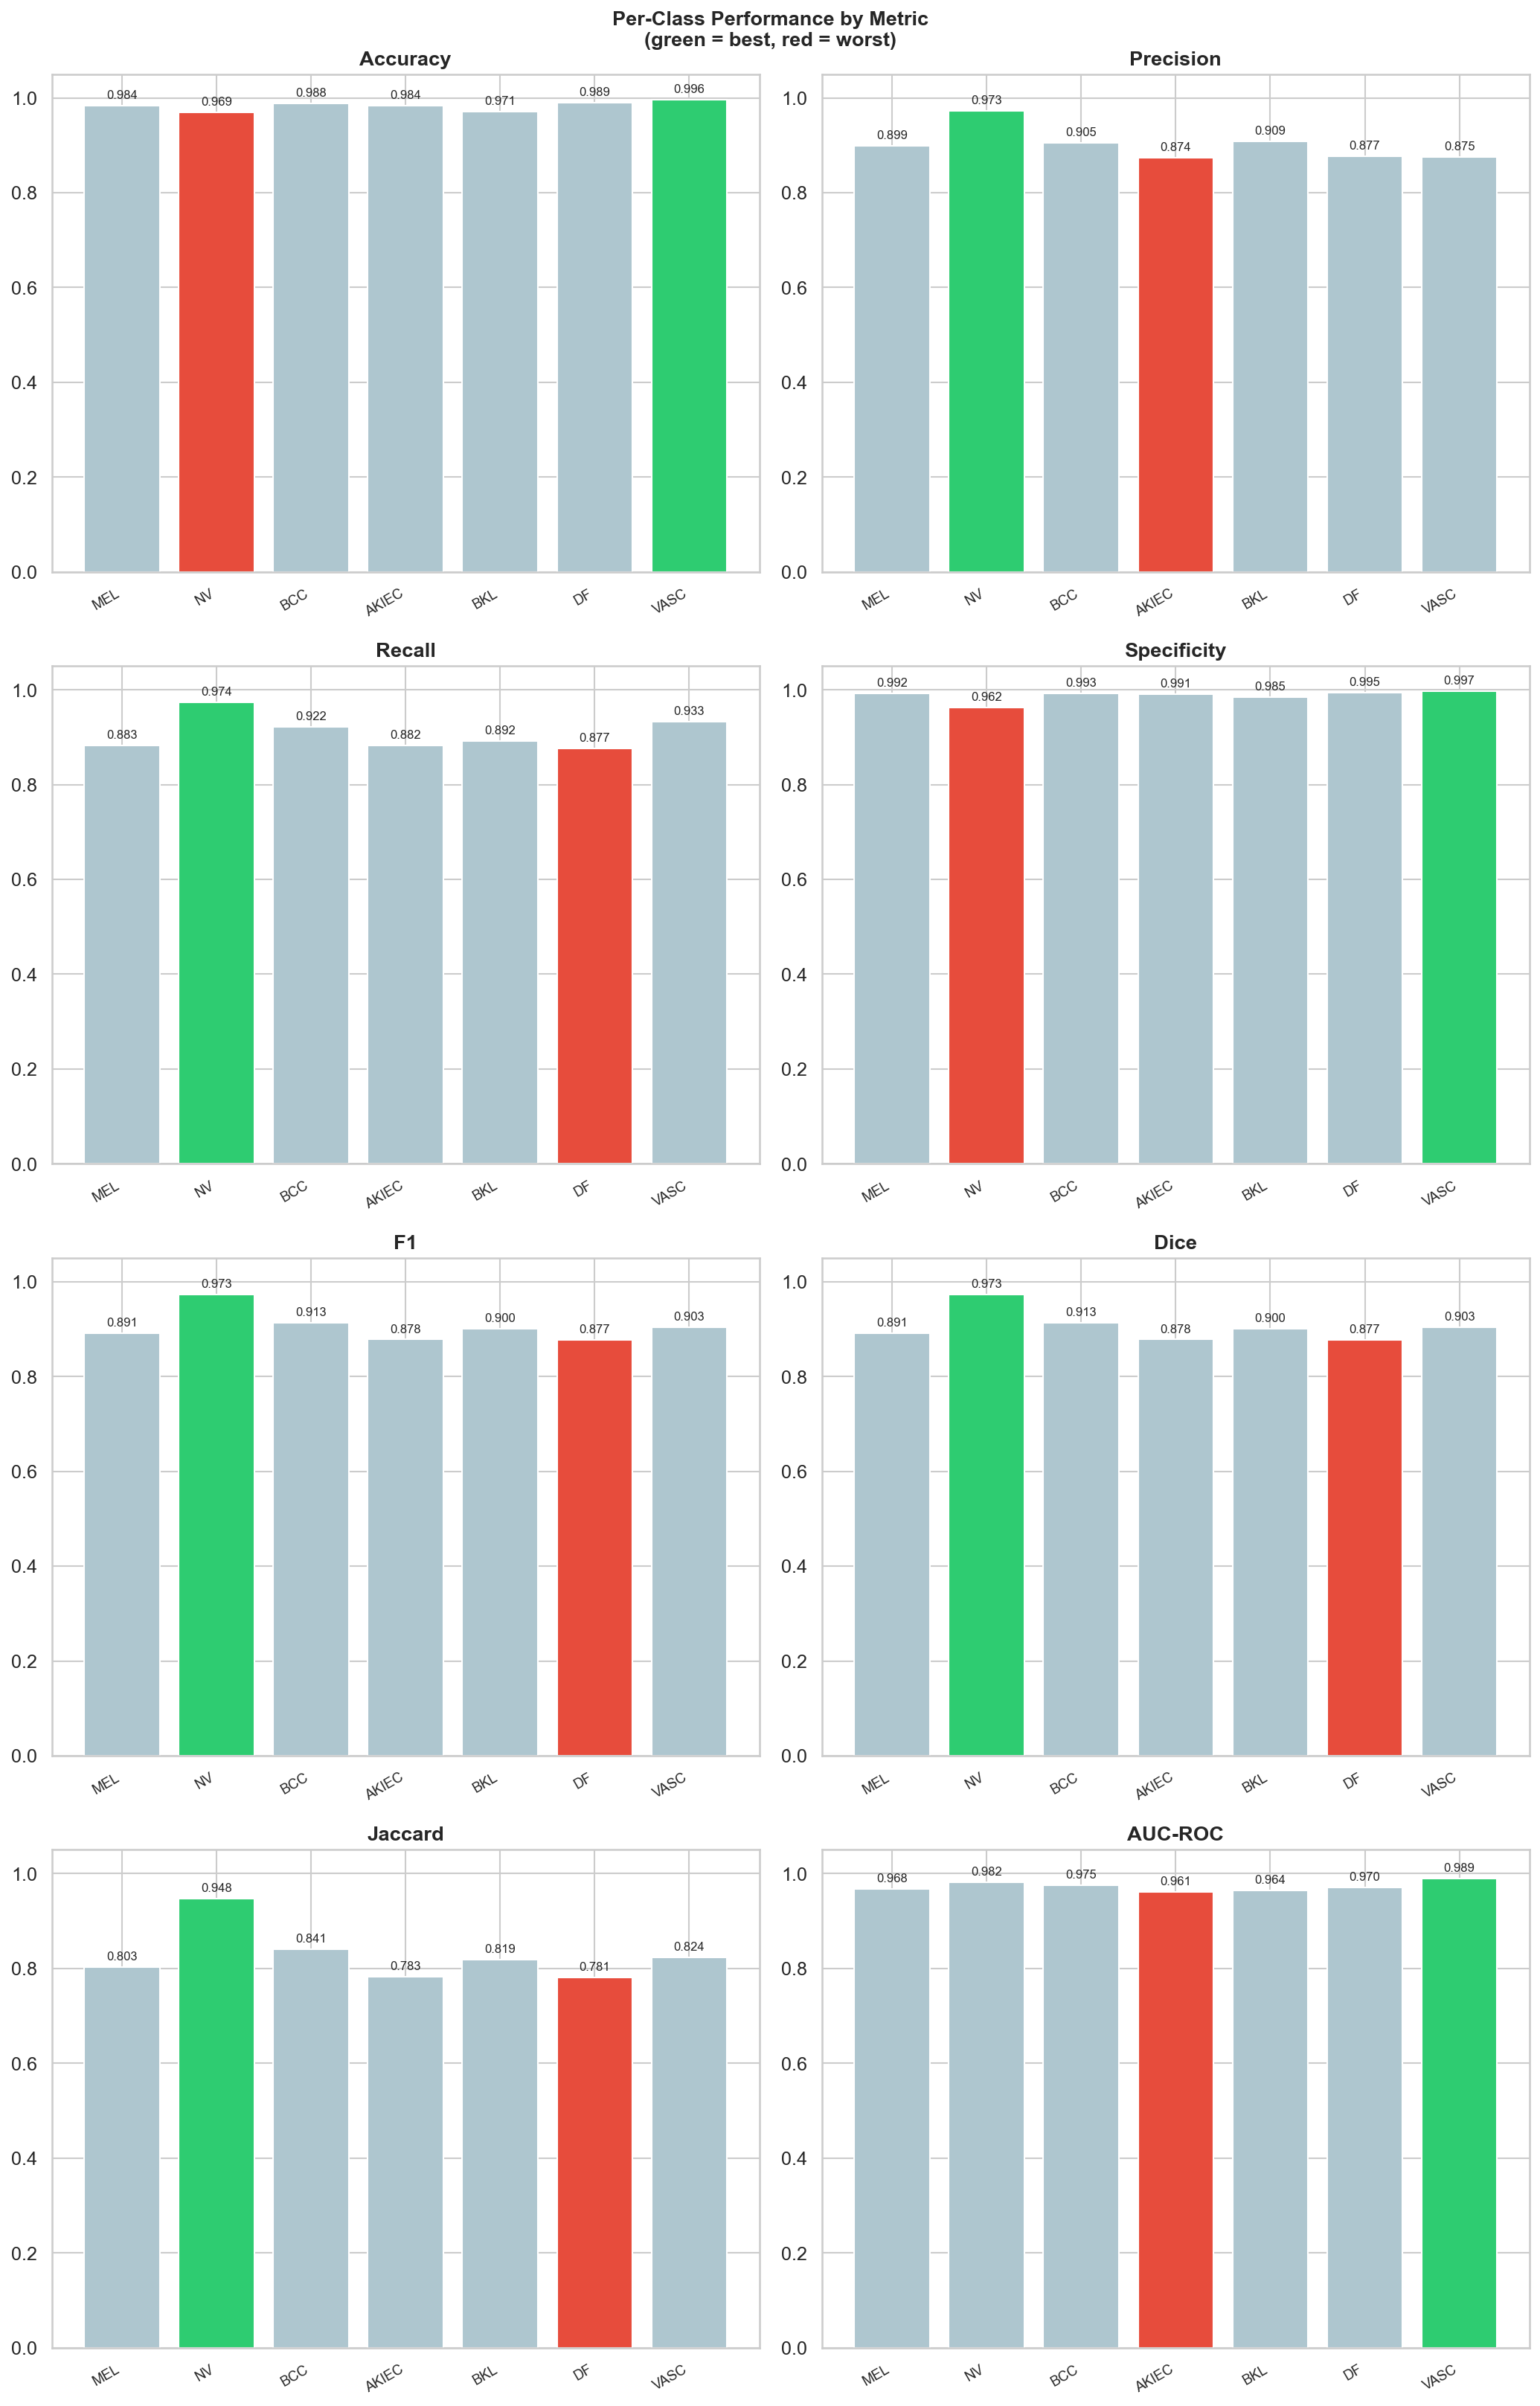
\includegraphics[width=0.9\textwidth]{per_metric_comparison.png}
  \caption{Per-metric class comparison (green = best, red = worst)}
  \label{fig:comp}
\end{figure}

\section{Class Ranking by F1}

\begin{table}[ht]
  \centering
  \caption{Class ranking by macro F1}
  \label{tab:rank}
  \begin{tabular}{clcc}
    \toprule
    \textbf{Rank} & \textbf{Class} & \textbf{F1} & \\
    \midrule
    1 & NV    & 0.9732 & \textit{Best} \\
    2 & BCC   & 0.9135 & \\
    3 & VASC  & 0.9032 & \\
    4 & BKL   & 0.9005 & \\
    5 & MEL   & 0.8909 & \\
    6 & AKIEC & 0.8780 & \\
    7 & DF    & 0.8769 & \textit{Worst} \\
    \bottomrule
  \end{tabular}
\end{table}

% ==========================================================
\chapter{Conclusion}
% ==========================================================

This project demonstrates that a DenseNet-121 classifier built \textbf{entirely from scratch using NumPy} — with no deep learning framework — can achieve strong results on a real-world medical imaging benchmark. The system reaches a macro F1 of \textbf{0.9052} and an AUC-ROC of \textbf{0.9729} on the ISIC 2018 Task 3 seven-class skin lesion classification task.

Key design decisions that drove performance:
\begin{itemize}
  \item \textbf{Weighted random sampling} and \textbf{focal loss} together address severe class imbalance without discarding data.
  \item \textbf{Two-phase training} (frozen backbone warm-up then full fine-tuning) prevents random-head destruction of feature representations in early epochs.
  \item \textbf{Cosine annealing} with a generous early-stopping patience of 12 epochs allows the optimiser to escape local minima while avoiding over-fitting.
  \item \textbf{Heavy dropout} (0.6) provides strong regularisation for a 7-million-parameter network trained on fewer than 10{,}000 images.
\end{itemize}

The preprocessing pipeline (Phase 1) contributes by supplying clean, hair-removed, contrast-enhanced images that let the classifier focus on true lesion morphology rather than artefacts.

\end{document}
